\documentclass[runningheads]{llncs}
\usepackage[T1]{fontenc}
\usepackage[utf8]{inputenc}
\usepackage{lmodern} 
\usepackage{graphicx}
\usepackage{amsmath,amssymb}
\usepackage{hyperref}
\usepackage{xcolor}
\usepackage{booktabs}
\usepackage{tabularx}
\usepackage{ragged2e}
\usepackage{array}
\usepackage{ltxtable}
\usepackage{longtable}
\usepackage{cite}

\newcolumntype{L}{>{\RaggedRight\arraybackslash}X}
\newcolumntype{P}[1]{>{\RaggedRight\arraybackslash}p{#1}}

\title{Personalized Healthcare with Artificial Intelligence: A Promising Future}

\author{Djelloul Daouadji Fadela \and Bachir Bouidjra Rochdi}
\institute{Department of Computer Science, University Mascara, Mascara, Algeria \\
\email{djellouldaouadji.f@univ-mascara.dz}
}


\begin{document}
\maketitle

\begin{abstract}
The rapid advancements in Artificial Intelligence (AI) are fundamentally transforming healthcare, moving towards a highly personalized paradigm that promises precision medicine tailored to individual patient characteristics. This comprehensive survey presents a novel data-centric categorization of AI applications in personalized healthcare, examining how different data modalities genomic, imaging, electronic health records, wearable sensors, and multimodal integration drive the development of personalized medical interventions. We systematically analyze current methodologies, highlighting the predominant use of Deep Learning and Reinforcement Learning across various healthcare domains, from personalized diagnostics and risk prediction to treatment optimization and drug therapy management. Despite significant progress demonstrated across many reviewed studies, persistent challenges including data quality and availability, model interpretability, clinical integration barriers, and ethical considerations continue to impede widespread adoption. Our analysis reveals promising future directions including explainable AI development, seamless clinical workflow integration, proactive preventive healthcare, and robust ethical governance frameworks. This survey contributes a unique perspective by emphasizing how the inherent characteristics of different data types fundamentally shape AI model development, deployment challenges, and personalization capabilities, ultimately underscoring AI's transformative potential to revolutionize patient care and enhance clinical outcomes.
\end{abstract}

\keywords{Personalized Healthcare, Artificial Intelligence, Deep Learning, Reinforcement Learning, Precision Medicine}

\section{Introduction}
The aspiration of personalized medicine, tailoring healthcare to an individual's unique characteristics, has been a long-standing goal in the medical field \cite{alum2025artificial}. This vision, which moves beyond a "one-size-fits-all" approach to consider a patient's molecular, physiological, ecological, and behavioral traits, has been significantly advanced by technological progress. The complete sequencing of the human genome in 2003 marked a pivotal moment, broadening personalized medicine's scope to encompass the entire spectrum of molecular medicine. More recently, Artificial Intelligence (AI) has emerged as a transformative force, actualizing this aspiration and profoundly changing healthcare by promising to improve diagnosis, treatment, patient care, and accelerate drug discovery \cite{alum2025artificial}. Despite the immense potential of AI in revolutionizing personalized care and enhancing overall clinical outcomes, ongoing challenges, including ethical considerations and the need for more relevant human-based models, continue to shape its development \cite{alum2025artificial,taherdoost2024ai}.

\section{Background}
The burgeoning field of Artificial Intelligence (AI) in personalized healthcare has led to a rich body of literature, with numerous surveys and reviews attempting to classify the diverse applications and methodologies. Understanding these existing categorization schemes is crucial to appreciating the unique contribution of our proposed approach.

\section{Related Work and Background}

\subsection{Evolution of AI-Driven Personalized Healthcare}
The intersection of AI and personalized healthcare has evolved through several key phases. Initially focused on basic pattern recognition in medical images, AI applications have expanded to encompass complex multimodal data integration for comprehensive patient profiling \cite{generative_ai_2024}. Recent advances in generative AI have further revolutionized the field by enabling synthetic data generation for training robust models while preserving patient privacy \cite{wang2024systematic}.

\subsection{Existing Categorization Approaches}
The burgeoning field of AI in personalized healthcare has led to a rich body of literature, with numerous surveys and reviews attempting to classify the diverse applications and methodologies. Understanding these existing categorization schemes is crucial to appreciating the unique contribution of our proposed approach.

Traditionally, previous works have adopted several prevalent methods for classifying AI applications in healthcare:

\begin{itemize}
    \item \textbf{Functional Role Categorization}: Many studies organize AI applications based on their functional utility within the healthcare ecosystem. This involves grouping applications into broad categories such as personalized diagnostics, risk prediction, treatment optimization, drug discovery, or patient management \cite{alum2025artificial,kumar2024artificial}. For instance, a common distinction is made between AI used for "personalized diagnostics and risk prediction" versus "personalized treatment optimization and management," reflecting key stages in clinical care \cite{article_1,article_18,article_2}.

    \item \textbf{AI Methodology-Based Categorization}: Another widely used approach categorizes studies by the specific AI techniques employed. This often differentiates between applications primarily leveraging Deep Learning (DL) for complex pattern recognition in high-dimensional data, Reinforcement Learning (RL) for sequential decision-making in dynamic environments, or traditional Machine Learning (ML) algorithms for predictive modeling \cite{article_22,article_23,article_18,article_11,ml_dl_advances_2023}.

    \item \textbf{Disease-Specific Categorization}: Some reviews focus on the impact of AI within specific disease areas or medical specialties. This involves detailing AI's contributions to fields such as oncology \cite{raza2024artificial,article_19}, cardiology \cite{article_6,article_8}, neurology \cite{article_3}, or chronic disease management \cite{article_9,article_2,article_22}.

    \item \textbf{Clinical Application-Based Categorization}: Recent comprehensive reviews have organized AI applications based on their primary clinical use cases, such as diagnostic support, treatment recommendation, drug discovery, or population health management \cite{singh2024comprehensive,ai_healthcare_transform_2023}.
\end{itemize}

\subsection{Gap in Current Literature}
While these existing categorization schemes offer valuable frameworks for understanding AI in personalized healthcare, they often discuss the data types implicitly rather than as a primary organizing principle. However, the inherent characteristics of the data its modality, volume, velocity, variety, and veracity are foundational to how AI models are developed, trained, and deployed for personalization \cite{ai_precision_medicine_2024}.

\subsection{Our Novel Data-Centric Approach}
For this paper, we propose a novel categorization based on the primary data modality utilized by the AI system. This data-centric approach offers a more granular and fundamental perspective, allowing us to:
\begin{itemize}
    \item Highlight how the nature of the input data dictates the choice of AI methodology
    \item Identify specific challenges (e.g., data sparsity, noise, interpretability) that are unique to or exacerbated by particular data types
    \item Emphasize how truly "personalized" healthcare is achieved by leveraging an individual's unique data profile, requiring AI systems capable of processing diverse and complex information
    \item Provide targeted recommendations for addressing modality-specific challenges
\end{itemize}

This perspective is crucial because personalized healthcare moves beyond general population statistics to individual patient characteristics, which are inherently captured in distinct data modalities \cite{precision_ai_future_2021}.

\subsection{Methodological Framework}
Our analysis follows systematic review principles adapted for AI healthcare research \cite{prisma_ai_guidelines_2023}, examining many key studies spanning genomic data analysis, medical imaging, electronic health records processing, wearable sensor integration, and multimodal data fusion approaches. Each study was evaluated based on its primary data modality, AI methodology, clinical application, reported outcomes, and identified challenges.

Table \ref{tab:data_centric_categorization} summarizes our proposed data-centric categorization, illustrating typical AI methods and associated challenges and benefits for each data modality.

\begin{table}[htbp]
    \centering
    \caption{Data-Centric Categorization of AI Applications in Personalized Healthcare}
    \label{tab:data_centric_categorization}
    \begin{tabularx}{\textwidth}{L L L L}
        \toprule
        \textbf{Data Modality} & \textbf{Typical AI Methods} & \textbf{Key Applications / Benefits} & \textbf{Associated Challenges} \\
        \midrule
        \textbf{Genomic \& Omics Data} & Deep Learning (CNN, RNN), Support Vector Machines, Random Forest, Feature Selection Algorithms & Personalized drug response prediction, pharmacogenomics, biomarker discovery, disease susceptibility assessment & High dimensionality, data sparsity, biological interpretability, population diversity bias \cite{article_1,rajesh2024transformative} \\
        \addlinespace
        \textbf{Medical Imaging Data} & Convolutional Neural Networks (CNNs), Vision Transformers, Generative Adversarial Networks (GANs), Transfer Learning & Diagnostic image analysis, tumor detection and classification, COVID-19 screening, anatomical segmentation & Data quality variability, annotation costs, model interpretability, generalization across imaging protocols \cite{article_11,article_12,article_20,article_23,article_21} \\
        \addlinespace
        \textbf{EHR \& Clinical Data} & Recurrent Neural Networks (RNNs), Transformers, Long Short-Term Memory (LSTM), Reinforcement Learning & Risk stratification, disease progression modeling, personalized treatment planning, clinical decision support & Data heterogeneity, missing values, temporal irregularities, privacy concerns, interoperability challenges \cite{article_2,article_13,article_18,article_24,article_10} \\
        \addlinespace
        \textbf{Wearable \& Sensor Data} & Time-Series Deep Learning (LSTM, GRU), Signal Processing, Anomaly Detection, Edge AI & Continuous health monitoring, early disease detection, personalized lifestyle interventions, real-time feedback systems & Signal noise, sensor drift, battery constraints, data privacy, real-time processing requirements \cite{article_3,article_4,article_6,article_9,article_22} \\
        \addlinespace
        \textbf{Multi-Modal Integration} & Multi-modal Deep Learning, Attention Mechanisms, Graph Neural Networks, Federated Learning, Digital Twin Architectures & Comprehensive patient profiling, holistic risk assessment, precision treatment selection, personalized care pathways & Data fusion complexity, computational scalability, model interpretability, cross-modal alignment challenges \cite{article_1,article_13,article_17,article_19} \\
        \bottomrule
    \end{tabularx}
\end{table}

This data-centric categorization enables a deeper exploration of the specific technical requirements, inherent biases, and interpretability challenges associated with each data type. Figure \ref{fig:data_centric_ai} visually illustrates how diverse data modalities form the foundation for AI-driven personalized healthcare.

\begin{figure}[h]
    \centering 
    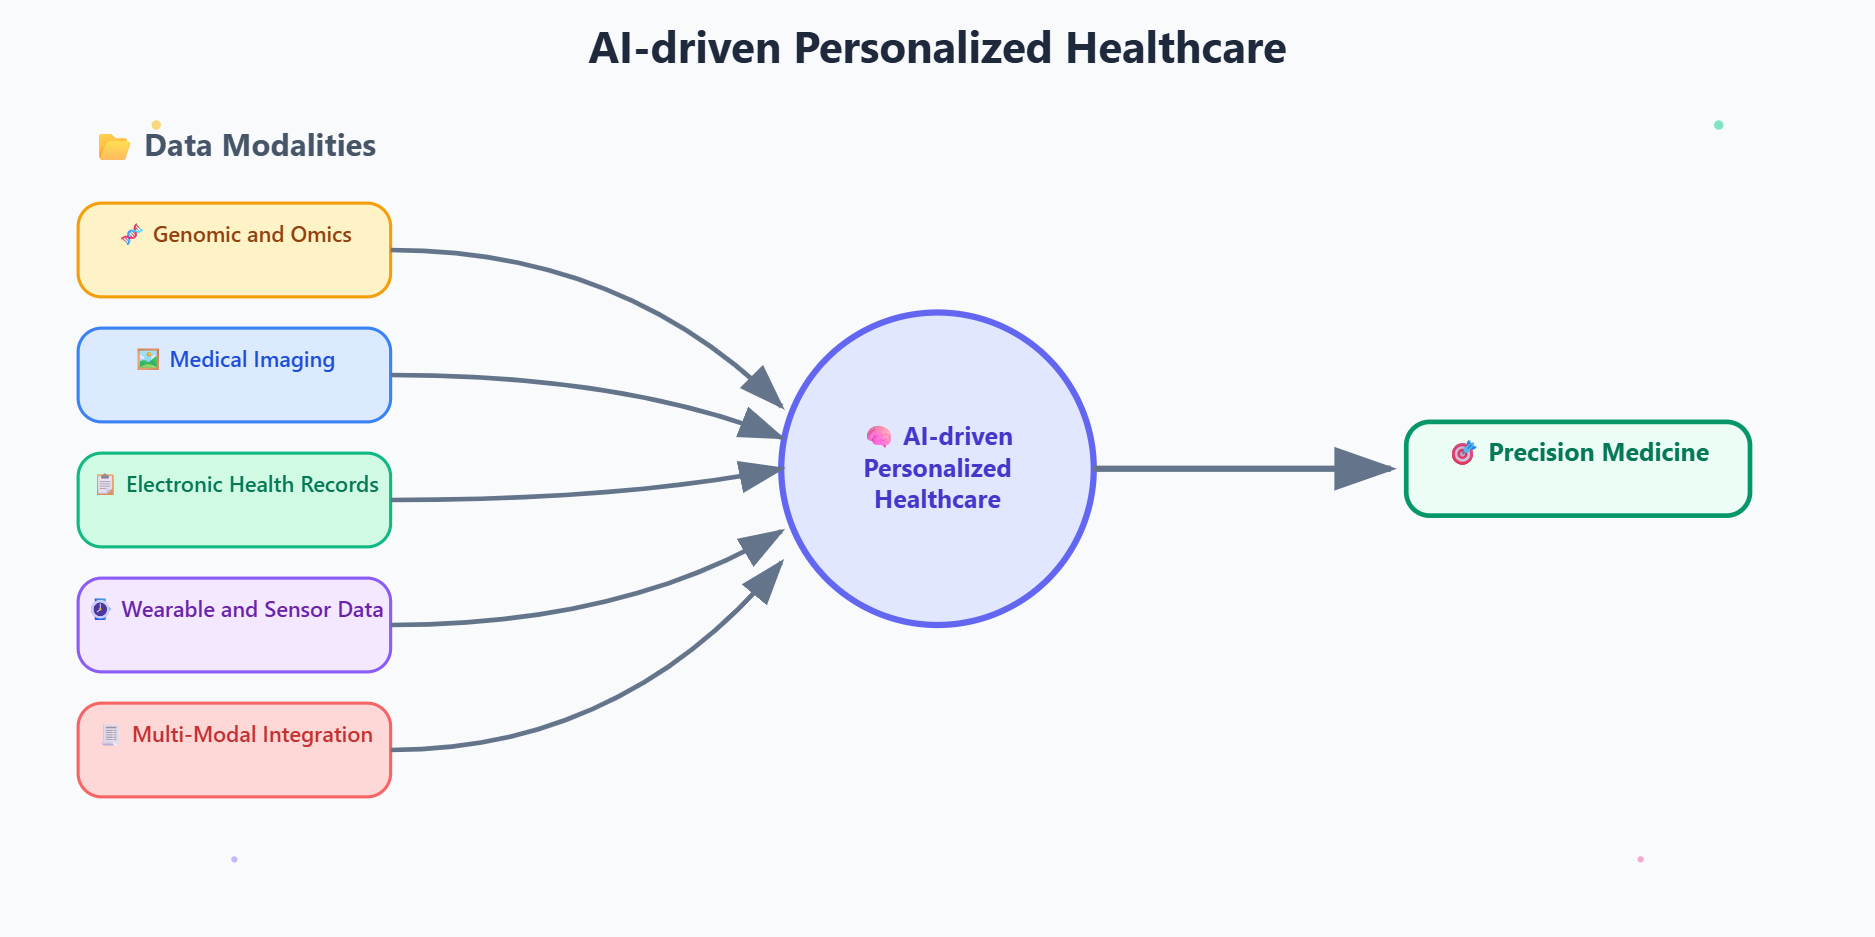
\includegraphics[width=1.0\textwidth]{multi_modal_data.png} 
    \caption{Multi-Modal Data Integration for Personalized Healthcare AI Systems. This diagram shows how diverse patient data modalities are processed through specialized AI models to enable personalized medical interventions with continuous feedback loops.}
    \label{fig:data_centric_ai}
\end{figure}

\section{Data-Centric Analysis of AI Applications}

\subsection{Genomic and Omics Data Applications}
Genomic data represents the foundation of precision medicine, offering unprecedented insights into individual genetic variations that influence disease susceptibility and drug responses \cite{rajesh2024transformative}. Our analysis reveals several key applications:

\textbf{Pharmacogenomics and Drug Response Prediction}: De Jong et al. \cite{article_1} demonstrated the potential of AI in predicting individual drug responses for epilepsy patients using genomic data, though their study was limited to 235 patients. The challenge of translating pharmacogenomic insights into clinical practice remains significant, with data sparsity and high dimensionality being primary concerns \cite{ai_pharmacogenomics_2024}. This area aims to predict how an individual will respond to specific drugs based on their genetic makeup, optimizing efficacy and minimizing adverse effects.

\textbf{Disease Susceptibility and Early Diagnosis}: AI models can analyze vast genomic datasets to identify genetic markers associated with increased risk for various diseases, including complex conditions like cancer, cardiovascular diseases, and neurodegenerative disorders. This enables proactive screening and early diagnostic interventions for at risk individuals, long before symptoms appear. For instance, machine learning algorithms are increasingly used to detect early signs of genetic predispositions to inherited cancers or to predict the onset of multifactorial diseases based on polygenic risk scores.

\textbf{Personalized Cancer Treatment (Oncology)}: In oncology, genomic and transcriptomic profiling of tumors allows for the identification of specific mutations or gene expression patterns that drive cancer growth. AI algorithms can then match these molecular signatures to the most effective targeted therapies or immunotherapies for an individual patient, moving beyond traditional one-size-fits-all chemotherapy. This approach significantly improves treatment outcomes and reduces unnecessary side effects.

\subsection{Medical Imaging Data Applications}
Medical imaging has been one of the most successful domains for AI implementation in healthcare, with applications ranging from diagnostic support to treatment planning \cite{article_21}.

\textbf{Diagnostic Imaging}: Kermany et al. \cite{article_21} demonstrated the power of deep learning in identifying medical diagnoses from retinal OCT images, achieving expert-level performance. Similarly, COVID-19 detection from chest X-rays and CT scans has shown promising results \cite{article_20,article_23}, though concerns about dataset bias and generalization remain.

\textbf{Advanced Applications}: Reinforcement learning applications in medical imaging, such as brain tumor localization \cite{article_12} and skin cancer diagnosis \cite{article_11}, represent emerging frontiers that combine diagnostic accuracy with treatment planning optimization.

\subsection{Electronic Health Records and Clinical Data}
EHRs represent a rich source of longitudinal patient data, enabling comprehensive health monitoring and predictive analytics \cite{article_10}.

\textbf{Risk Prediction and Disease Modeling}: Machine learning approaches for diabetes prediction using EHR data have shown significant promise \cite{article_2}, with explainable AI techniques improving clinical acceptance. Deep Q-networks have been successfully applied to disease prediction tasks \cite{article_10}, demonstrating the potential of reinforcement learning in clinical decision support.

\textbf{Personalized Treatment Planning}: Reinforcement learning applications in treatment optimization, such as personalized multimorbidity management for Type 2 diabetes patients \cite{article_18} and sepsis treatment protocols \cite{article_13}, represent significant advances in precision medicine.

\subsection{Wearable and Sensor Data Applications}
The proliferation of wearable devices has created new opportunities for continuous health monitoring and early intervention \cite{article_9}.

\textbf{Continuous Glucose Monitoring}: Anjum et al. \cite{article_9} demonstrated the potential of AI-enhanced time series analysis for personalized dietary interventions in Type 2 diabetes management. The integration of continuous glucose monitoring data with AI algorithms enables real-time treatment adjustments.

\textbf{Cardiovascular Monitoring}: Heart sound classification using deep learning \cite{article_6} and ECG-based diabetes detection \cite{article_4} showcase the potential of wearable sensors for early disease detection and continuous monitoring.

\textbf{Artificial Pancreas Systems}: The development of safe-enhanced closed-loop artificial pancreas controllers \cite{article_22} represents a pinnacle of wearable sensor integration with AI, demonstrating real-time personalized treatment delivery.

\subsection{Multi-Modal Data Integration}
The future of personalized healthcare lies in the integration of multiple data modalities to create comprehensive patient profiles \cite{generative_ai_2024}.

\textbf{Digital Twin Approaches}: Patient-physician digital twin dyads for cancer treatment optimization \cite{article_17} represent an advanced form of multi-modal integration, combining clinical data, imaging, and treatment response information for personalized therapy selection.

\textbf{Comprehensive Risk Assessment}: Multi-modal approaches enable holistic patient profiling that considers genetic predisposition, lifestyle factors, clinical history, and real-time physiological data for comprehensive risk assessment and personalized intervention strategies.

\section{Comprehensive Challenges and Limitations}

\subsection{Data-Related Challenges}
\begin{itemize}
    \item \textbf{Limited Dataset Size \& Diversity}: The scarcity of large, diverse, and representative datasets significantly impedes the generalizability and robustness of AI models. This limitation is evident in studies such as epilepsy drug response prediction (only 235 patients) \cite{article_1}, diabetes detection with limited ECG subjects \cite{article_4}, COVID-19 CT scans (1,065 images) \cite{article_20}, brain tumor MRI (60 images) \cite{article_12}, and the artificial pancreas (30 simulated patients) \cite{article_22}.
    \item \textbf{Data Sparsity \& Missing Values}: High-dimensional but sparse data, particularly from genomics or Electronic Health Records (EHRs), complicates effective feature extraction. Examples include genomic data sparsity in epilepsy \cite{article_1}, challenges with missing insulin values in diabetes studies \cite{article_2}, and missing gait metrics in Alzheimer's research \cite{article_3}.
    \item \textbf{Data Heterogeneity \& Noise}: Variability stemming from diverse data sources (e.g., different sensors, imaging protocols) inherently affects model robustness and reliability. This can be seen in ECG-based diabetes detection (e.g., HRV signal noise) \cite{article_4}, PCG-based heart sound classification (acoustic variability) \cite{article_6}, and inconsistencies within ICU data for mechanical ventilation optimization \cite{article_24}.
\end{itemize}

\subsection{Model-Related Challenges}
\begin{itemize}
    \item \textbf{Interpretability \& Trust ("Black Box" Problem)}: The inherent lack of transparency in many deep learning models and complex Reinforcement Learning systems hinders clinical adoption and trust, as clinicians need to understand the rationale behind AI-driven decisions. This challenge is prominent in models like CNN-RNN for Alzheimer's gait analysis \cite{article_3}, Deep Q-learning for diabetes management \cite{article_11,article_22}, and RL approaches for skin cancer diagnosis \cite{article_11}.
    \item \textbf{Overfitting \& Generalization Issues}: AI models may exhibit strong performance on training data but frequently fail to generalize consistently to new, unseen real-world patient populations or clinical settings. Examples include concerns about dataset bias in COVID-19 X-ray detection \cite{article_23}, reliance on small private datasets for diabetes prediction \cite{article_2}, and the persistent simulation-to-reality gap in reinforcement learning for sepsis treatment \cite{article_13}.
    \item \textbf{Computational Complexity}: Resource-intensive training and deployment requirements for advanced AI models limit their practical application, especially in low-resource healthcare settings or for real-time inference. This affects models such as hybrid CNN-RNN models \cite{article_3}, Deep Q-networks for brain tumor localization \cite{article_12}, and real-time artificial pancreas control \cite{article_22}.
\end{itemize}

\subsection{Clinical \& Practical Challenges}
\begin{itemize}
    \item \textbf{Integration into Clinical Workflows}: A significant barrier is the lack of seamless interoperability with existing Electronic Health Records (EHRs) and potential resistance from clinicians to adopt new AI tools. This impacts the practical utility of AI-based drug response prediction \cite{article_1}, RL for ventilator settings \cite{article_24}, and the real-world deployment of explainable diabetes tools \cite{article_2}.
    \item \textbf{Regulatory \& Ethical Barriers}: The development of AI-based medical devices faces stringent validation requirements, necessitating clear regulatory pathways and robust ethical considerations. This is critical for areas like epilepsy biomarker models \cite{article_1}, closed-loop insulin delivery systems \cite{article_22}, and AI-powered COVID-19 diagnostics \cite{article_20,article_23}.
    \item \textbf{Safety \& Risk Management}: For life-critical applications in healthcare, such as those involving sepsis treatment or mechanical ventilation, absolute safety and fail-safe designs are paramount. This is a crucial concern for RL-based ICU interventions \cite{article_13,article_24} and for managing the risk of severe hypoglycemia with artificial pancreas systems \cite{article_22}.
\end{itemize}

\subsection{Patient-Specific Limitations}
\begin{itemize}
    \item \textbf{Individual Variability}: The inherent biological diversity among patients complicates the development of truly personalized recommendations and models that are robust across all individuals. This is particularly challenging in areas like diabetes, due to significant glucose response variability \cite{article_9}, and in cancer therapy, given tumor heterogeneity \cite{article_19}.
    \item \textbf{Longitudinal Data Gaps}: A common limitation is the insufficient availability of long term follow up data, which is crucial for effective chronic disease management and accurately tracking disease progression over time. This impacts research in areas like Alzheimer's progression tracking \cite{article_3} and personalized multimorbidity management for Type 2 Diabetes \cite{article_18}.
\end{itemize}

Figure \ref{fig:challenges} illustrates the multifaceted nature of these challenges and their interrelationships.

\begin{figure}[h]
\centering
    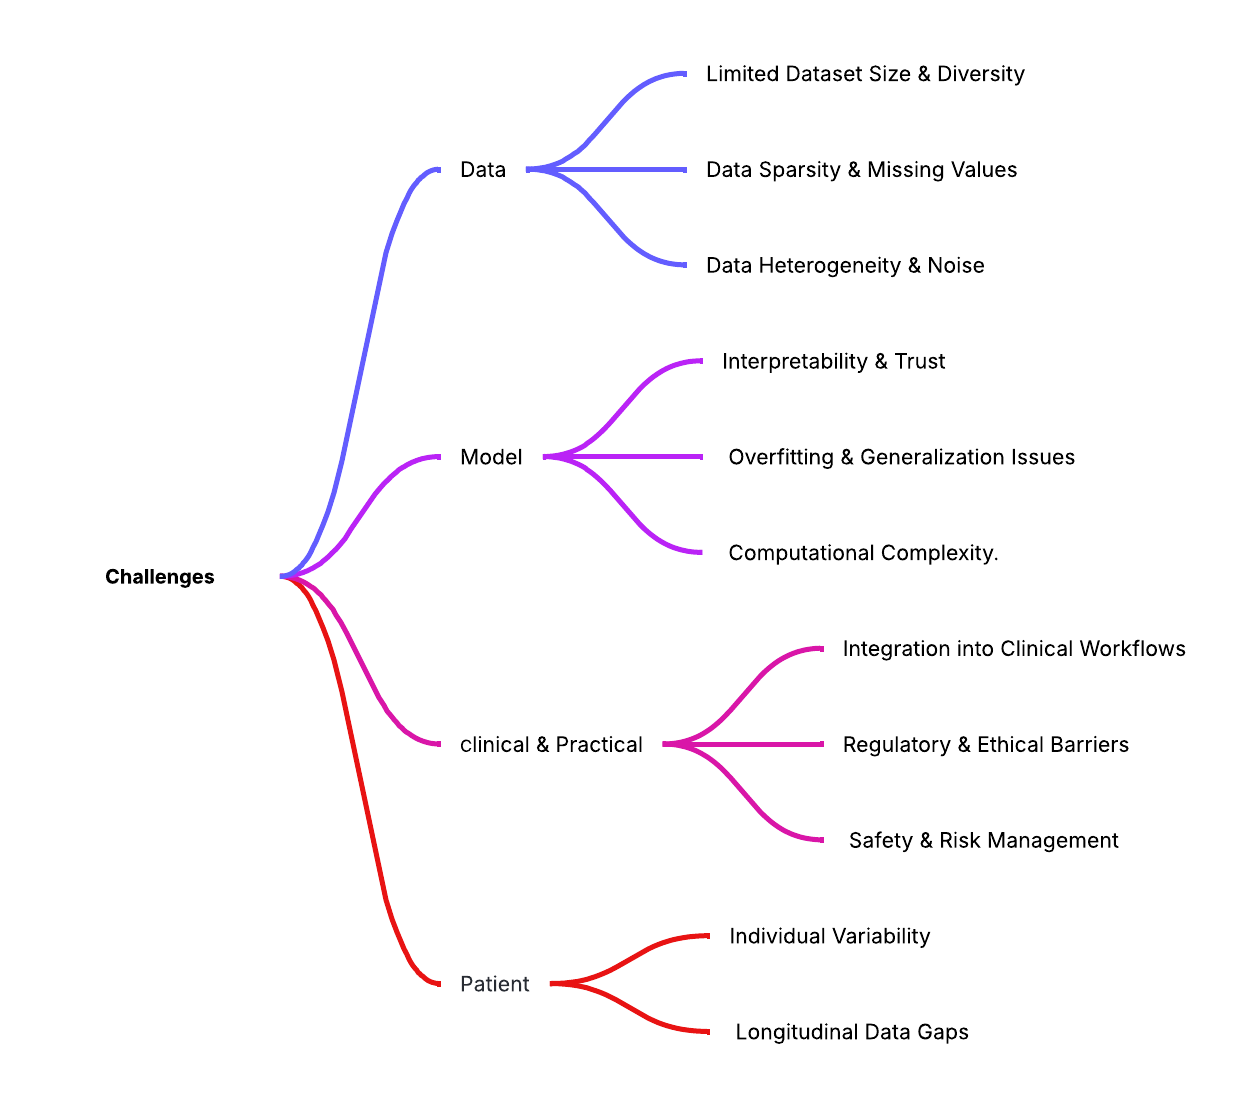
\includegraphics[width=0.8\columnwidth]{challenges.png}
    \caption{Interconnected Challenges in AI-Driven Personalized Healthcare. This diagram illustrates the interconnected nature of data-related, model-related, clinical, and ethical challenges that must be addressed for successful AI implementation in personalized healthcare.}
    \label{fig:challenges}
\end{figure}

\section{The Promising Future: Opportunities and Directions}
The trajectory of AI in personalized healthcare remains highly promising, with ongoing research and development focused on overcoming current limitations and unlocking new capabilities. The reviewed articles highlight several common themes and specific recommendations for advancing AI in personalized healthcare, often directly addressing the aforementioned challenges. These future directions can be categorized as follows:

\subsection{Multi-Modal Data Integration}
The future lies in fusing diverse data types genomics, proteomics, imaging, EHRs, and real-time wearable device data \cite{article_9, article_10} to create comprehensive "digital twins" of patients. This approach will enable truly holistic and hyper-personalized care by leveraging a complete picture of an individual's health \cite{article_17, article_19}. Patient-physician digital twin dyads for cancer treatment optimization \cite{article_17} represent an advanced form of multi-modal integration, combining clinical data, imaging, and treatment response information for personalized therapy selection.

\subsection{Advancements in Safe and Explainable AI (XAI)}
Research is actively developing new AI algorithms that are inherently more transparent, interpretable, and incorporate robust safety constraints. The dual safety mechanism in \cite{article_22} is an excellent example of this critical direction, directly addressing the "black box" problem and safety concerns. Explainable AI techniques are already showing promise in improving clinical acceptance, as demonstrated in diabetes prediction using EHR data \cite{article_2}.

\subsection{Proactive and Preventive Healthcare}
AI will increasingly shift the focus from reactive treatment to proactive disease prevention. This will be achieved through sophisticated risk stratification and personalized interventions tailored to an individual's predicted vulnerabilities, leveraging predictive analytics to intervene before disease onset. Continuous glucose monitoring with AI-enhanced time series analysis for personalized dietary interventions \cite{article_9} exemplifies this preventive approach in diabetes management.

\subsection{Seamless Integration and Interoperability}
Efforts to integrate AI solutions seamlessly into existing clinical workflows and to improve data interoperability across disparate healthcare systems will be crucial for widespread adoption \cite{muhammad2024artificial, singh2024comprehensive}. This will directly address the practical challenges of integrating new technologies into established medical practices, including the lack of seamless interoperability with existing Electronic Health Records (EHRs) and potential resistance from clinicians to adopt new AI tools.

\subsection{Ethical AI Governance and Policy}
The development of clear ethical guidelines, best practices, and agile regulatory frameworks will be essential to foster responsible innovation and build public trust in AI applications within healthcare. This directly responds to the regulatory and ethical barriers identified, including stringent validation requirements for AI-based medical devices \cite{article_20, article_21}.

\subsection{Human-AI Collaboration}
The future envisions AI as an intelligent assistant, augmenting the capabilities of healthcare professionals, rather than replacing them. Fostering a collaborative ecosystem where AI provides data-driven insights to support human decision-making will lead to optimal patient outcomes. This collaborative approach is essential for addressing the interpretability challenge and building trust between clinicians and AI systems \cite{future_healthcare_professionals_2024}.

\section{Discussion}
This review highlights AI's role in personalized healthcare, emphasizing a data-driven paradigm. Challenges, from data limitations to interpretability and clinical integration, are deeply linked to data modalities. Genomic and omics data face sparsity and high dimensionality, while imaging and sensor data demand robust preprocessing. The "black box" problem particularly impedes models trained on complex multi-modal datasets.

A significant gap exists between AI's theoretical potential and its widespread adoption, not just technically but also due to regulatory, ethical, and sociological hurdles. A lack of standardized ethics and clear regulatory pathways, coupled with clinician resistance stemming from trust issues and safety concerns, hinder deployment.

Future directions directly address these challenges. Multi-modal data integration, building "digital twins," aims to overcome single-modality limitations by providing richer input, though it introduces new harmonization challenges. Advancements in Safe and Explainable AI (XAI), exemplified by dual safety mechanisms \cite{article_22}, are crucial for trust and safety in critical applications. The focus shifts to interpretable, actionable insights to foster human-AI collaboration.

AI's move towards proactive and preventive healthcare, leveraging predictive analytics for early intervention, promises better outcomes but requires models that generalize across diverse populations. Ultimately, seamless clinical integration and robust ethical governance, through collaboration among researchers, clinicians, and policymakers, are foundational to realizing personalized medicine.

\section{Conclusion}
This comprehensive survey presents a novel data-centric perspective on AI applications in personalized healthcare, moving beyond traditional functional or methodological categorizations to emphasize how different data modalities fundamentally shape AI development and deployment. The integration of Artificial Intelligence into personalized healthcare marks a transformative era, promising a future where medical interventions are precisely tailored to each individual \cite{alum2025artificial}. As this survey demonstrates, AI is already making significant strides in personalized diagnostics, risk prediction, and treatment optimization across various diseases, leveraging methodologies like Deep Learning and Reinforcement Learning. While challenges related to data, safety, interpretability, and ethics persist, ongoing research and collaborative efforts are actively addressing these hurdles \cite{taherdoost2024ai}. The continuous evolution of AI, coupled with the increasing availability of diverse patient data, points towards a highly promising horizon where personalized healthcare becomes more accessible, effective, and truly patient-centric, ultimately enhancing global health outcomes.

\bibliographystyle{splncs04}
\bibliography{references}

\end{document}